\documentclass[letterpaper,11pt]{article}

\usepackage{spverbatim}
\usepackage{minted}
\usepackage{amssymb}
\usepackage{bm}
\usepackage{graphicx}
\usepackage{amsmath}

\usepackage{minted}
\usepackage{titling}
\newcommand{\subtitle}[1]{%
  \posttitle{%
    \par\end{center}
    \begin{center}\LARGE#1\end{center}
    \vskip0.5em}%
}

\usepackage{tabularx} % extra features for tabular environment
\usepackage{amsmath}  % improve math presentation
\usepackage{graphicx} % takes care of graphic including machinery
\usepackage[margin=1in,letterpaper]{geometry} % decreases margins
\usepackage{cite} % takes care of citations
\usepackage[final]{hyperref} % adds hyper links inside the generated
% pdf file
\usepackage{subcaption}
\usepackage{placeins}
%% \usepackage{placeins}

%% \hypersetup{
%% 	colorlinks=true,       % false: boxed links; true: colored links
%% 	linkcolor=blue,        % color of internal links
%% 	citecolor=blue,        % color of links to bibliography
%% 	filecolor=magenta,     % color of file links
%% 	urlcolor=blue
%% }
%++++++++++++++++++++++++++++++++++++++++

\title{\textbf{EECE 5639, Extra Credit Project:
\\{\Large Stereo}}}
\author{Sreejith Sreekumar}
\date{\today}

\begin{document}

\maketitle

\begin{abstract}
  In traditional stereo vision, two cameras, displaced horizontally from one another are used to obtain two differing views on a scene. By comparing these two images, the relative depth information can be obtained in the form of a disparity map, which encodes the difference in horizontal coordinates of corresponding image points. The values in this disparity map are inversely proportional to the scene depth at the corresponding pixel location. Building on these ideas we try to estimate the depth of a scene.
 \end{abstract}


\section{Description of Algorithms}
In this section we list and describe all of the algorithms implemented in the completion of this
project.

\subsection{Corner Detection}
Harris Corner Detector is a corner detection operator that is commonly used in computer vision algorithms to extract corners and infer features of an image. This algorithm takes the differential of the corner score into account with reference to direction directly. The main equations in corner detection are given by:

\begin{itemize}
\item  Computation of M from gradient components
\[
  M = \sum\limits_{x,y} w(x,y)
    \begin{bmatrix}
      I_{x}^{2} & I_{x}I_{y} \\
      I_{x}I_{y} & I_{y} ^{2}
    \end{bmatrix}
\]
\item Intensity change in shifting window eigenvalue analysis:
\[
E(u, v) =
    \begin{bmatrix}
      u & v \\
    \end{bmatrix}
    \]
\item Corner Response Measure

\[
 R = det M - k\ trace^{2}(M)
\]

\item Threshold R to determine the corners.

\end{itemize}


\subsection{Non-Max Suppression}
The output of harris corner detection could be thought of as a heat
map, with a region of high magnitudes around a single corner. In order
to produce corners from this map, we define the local maxima within a
region as a corner, if it is above a certain threshold. To find these
local maxima we slide a 3x3 window over the image. Every pixel in the
window that is less then than maximum value in the window is set to
zero.

\subsection{Normalized Cross Correlation}
We use the corners as features to find the interesting points in each
image and determine pair-wise point correspondences. One of the
methods to compare these interesting regions is Normalized Cross Correlation. \\

Normalized Cross Correlation is defined by the equation:
\[
N_{fg}  = \sum\limits_{x,y} \hat{f}(i,j)\hat{g}(i,j)
\]
where
\[
  \hat{f} = \frac{f}{||f||} = \frac{f}{\sqrt{\Sigma_{[i,j] \in R} f^{2}(i,j)}}
  \]

\[
  \hat{g} = \frac{g}{||g||} = \frac{g}{\sqrt{\Sigma_{[i,j] \in R} g^{2}(i,j)}}
  \]
  In practice, we perform a brute force search between all possible
  combinations of points from both images. We then sort the results of
  this search by magnitude of correlation value. The N correspondences
  with the highest normalized correlation values are maintained. The
  resulting correspondences are then further pruned by realistic
  geometric constraints. In our case, we know the images represent a
  small lateral rotation. Correspondences with vertical translations
  greater than a small threshold, or lateral translations greater than
  a large threshold are said to not fit this constraint, and are
  deleted. The result is approximately 60 robust correspondences
  between the two images.
  
  \subsection{Fundemental Matrix}
  The fundamental matrix is a 3 x 3 matrix which relates corresponding points in stereo images. In epipolar geometry
  with homogeneous image coordinates, x and x' of corresponding points in a stereo image pair, F * x describes a line
  on which the corresponding point x' must line (epipolar line). \\
  The equation relating x, x' and F can be written as
\[
  x'^{T} F x = 0
  \]
\subsection{Disparity Map}
  
  

\section{Experiments}
This section describes the intermediate steps and experiments
performed in the completion of this project.

\subsection{Reading the image inputs}

\subsection{Detecting Corners in the Images}
For both images, we apply the harris corner detection algorithm and then perform non max
supression and thresholding to get the co-ordinates of the corners
from the images. \\

Iterating through the corners detected for each image, we create
cropped neighborhoods for every corner with it at the center.
This way, we'd have N template patches corresponding to the N points
in the image which were detected to be corners. \\

Following this procedure, we do \textit{normalized cross correlation}
(subsection 1.3) on every template from the first image with every
other template of the second image, constituting a brute force search
of all point neighborhood correlation combinations between the
images. The results of this search are sorted by cross correlation
magnitude and all matches above a tuned correlation threshold are
kept.

The resulting matches are then pruned by realistic geometric
constraints. In our case, we know the images are both taken from the
same viewpoint from a slightly different angle. Thus we eliminate
correspondences with vertical translations above a small threshold and
lateral translations above a large threshold, to produce a set of
robust and realistic correspondences.\\


The correspondences which were found hence are visualized below using lines of different
colors.

\begin{figure}[h]
  \centering
  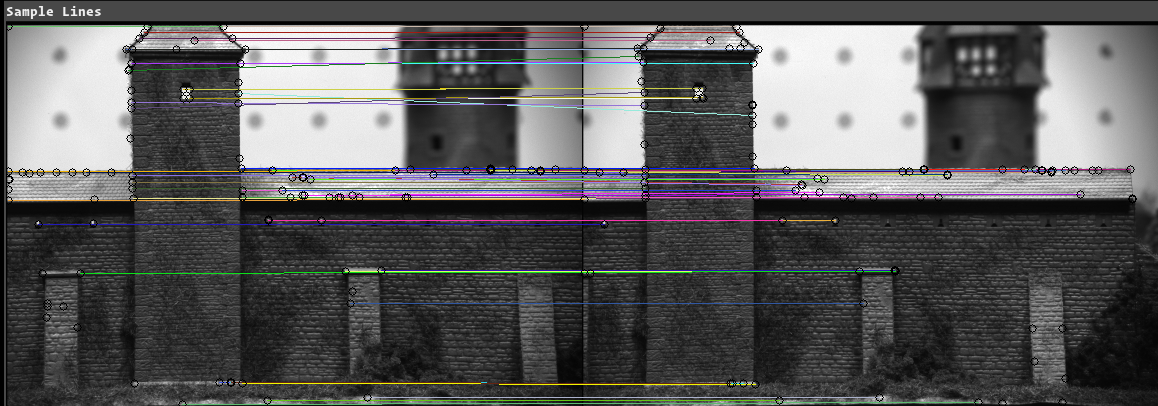
\includegraphics[width=\linewidth]{images/correspondences.png}
  \caption{Color Coded Corner Correspondences}
  \label{fig:sfig1}
\end{figure}



\section{Conclusion}


\section{Appendix}

\end{document}
